% -*- Mode: LaTeX; TeX-PDF-mode: t; -*-  # Config emacs auctex
\input{./._relpath-to-latexroot.ltx}    % Set paths to find resources (defines \latexroot and loads tex-paths.ltx)

\documentclass[titlepage, headings=optiontotocandhead]{econark} % embedded toc

% Definitions unique to this paper (showlabels config now in local.sty)
\usepackage{local}                % Local package definitions and setup
\usepackage{local-qe}             % local-qe gets pkgs req for qe

\bibliographystyle{plainnat}

% Load metadata BEFORE hypersetup (SST pattern)
\input{\latexroot/@local/metadata.ltx}

% When compiling Web version of paper, construct targets/anchors
\weborpdf{ % compiling web version
  \hypersetup{destlabel=true} % set up html labels
}{
  \provideboolean{showPageHead}{\setboolean{showPageHead}{true}}
  \hypersetup{
    pdftitle={\PDFTitle},
    pdfauthor={\PDFAuthor},
    pdfsubject={\PDFSubject},
    pdfkeywords={\PDFKeywords}
  }
}

\webonly{
  \section*{Endnotes}
  \theendnotes
}

\begin{document}

%% ----- Title page -----
\webonly{
  \newcommand{\versn}{Web}
}

\title{A Replication of Low (2005): Self-Insurance in a Life-Cycle Model of Labour Supply and Savings}

\author{REMARK Replication Package}

\keywords{Precautionary saving; Life-cycle labour supply}

\jelclass{D91; H31}

\date{}

\maketitle
\vspace{-0.5\baselineskip}

\whenintegrated{\label{abstract}} % integrated doc: SST for labels
\begin{abstract}
  \AbstractText
\end{abstract}
\vspace{-0.5\baselineskip}

This document is a REMARK-style replication note for Low (2005). Its purpose is to pair a
concise summary of the paper with executable code that reproduces the main quantitative
comparisons. In this repository, the computational replication is implemented in
\path{Code/Python/Low2005.py}.

\whenintegrated{\label{links}} % integrated doc: SST for labels

\providecommand{\REMARK}{\href{https://github.com/econ-ark/REMARK}{REMARK}}
\begin{footnotesize}
  \setlength{\parskip}{0pt}
  \parbox{0.9\textwidth}{
    \begin{tabbing}
      \texttt{~~~~~~~~~~~~~~~~~~~~~~~} \= \=  \\
      \texttt{~~~~GitHub~Repo:~~~~~~~} \> \> \texttt{\href{https://github.com/\owner/\projectname}{https://github.com/\owner/\projectname}} \\
      \texttt{~~~~~~~~~~~~~~~~~~~~~~~} \> \>  \\
      \texttt{~~~~Other~Materials:~~~} \> \> \\
      \texttt{~~~~~Replication~code:~} \> \> \texttt{\href{https://github.com/\owner/\projectname/tree/main/Code/Python}{Code/Python}} \\
    \end{tabbing}
  }
\end{footnotesize}
\vspace{-0.3\baselineskip}

\pagenumbering{gobble}

\titlepagefinish

\pagebreak

% Table of contents; to omit, \setboolean{TOC}{false} above
\ifthenelse{\boolean{TOC}}{\pagebreak
  \let\LaTeXStandardContentsName\contentsname
  \renewcommand{\contentsname}{}
  \tableofcontents
}{}

\section{Summary}
Low (2005) studies how households self-insure over the life cycle when future wages are
uncertain and markets are incomplete \cite{Low2005}. The paper's central point is that labour
supply is itself an insurance margin: if households can change hours worked, then they can
respond to wage risk using both savings and labour effort rather than savings alone.

This REMARK summarizes the paper briefly while leaving the main computational work to the
accompanying code. The Python implementation reproduces the paper's core comparisons
between certainty and uncertainty and between flexible and fixed labour supply.

The main economic conclusions are straightforward. Under uncertainty, households work more
and consume less early in life. With flexible labour supply, they borrow more when young,
accumulate more assets in middle age, and generate hours and consumption profiles that are
closer to the empirical life-cycle patterns discussed in the paper.

\section{Model Setup}
The model is a partial-equilibrium life-cycle problem in which households choose consumption,
leisure, and savings subject to wage risk. Period utility takes the Cobb--Douglas CRRA form
\begin{equation}
  u(c_t,l_t)=\frac{\left(c_t^{\eta} l_t^{1-\eta}\right)^{1-\gamma}}{1-\gamma}.
\end{equation}

Assets evolve according to
\begin{equation}
  A_{t+1}=(1+r)\left[A_t + (H-l_t)w_t - c_t\right],
\end{equation}
where $H-l_t$ is hours worked. The wage process combines a deterministic age profile with
permanent and transitory shocks:
\begin{align}
  \ln w_t &= \ln w_0 + \alpha_1 t + \alpha_2 t^2 + \ln w_t^P + \nu_t, \\
  \ln w_t^P &= \ln w_{t-1}^P + \varepsilon_t.
\end{align}

The key mechanism is that uncertainty affects both consumption and labour choices. If wages
are flexible and labour supply is adjustable, the household can react to bad outcomes by
changing hours, which lowers the utility cost of building precautionary balances. This is what
distinguishes the model from fixed-hours precautionary-savings frameworks such as
\cite{Deaton1991Low, GourinchasParker2002Low, Cagetti2003Low}.

\section{Calibration and Computation}
The paper calibrates the model at annual frequency and chooses the discount factor and the
utility weight on leisure to match average male hours and median wealth accumulation over
working life. The wage process moments are drawn from estimates in \cite{MeghirPistaferri2004Low},
and the key baseline values reported in the paper are summarized below.

\begin{table}[htbp]
  \centering
  \caption{Baseline calibration: common parameters as reported in Low (2005),
  and the discount rate~$\delta$ calibrated separately for each
  scenario by matching working-life median~$A/Y$ to the PSID 1995
  target of $1.84$. The first column of the second panel reproduces
  Low (2005), Table~1, p.~956; the second column reports the values
  obtained by the bisection search in
  \protect\path{Code/Python/Low2005.py}.}
  \label{tab:calibration}
  % AUTO-GENERATED by Code/Python/Low2005.py - do not edit by hand.
\begin{tabular}{lc}
\toprule
\multicolumn{2}{l}{\textit{Common parameters (held fixed across scenarios)}} \\
\midrule
Parameter & Value \\
\midrule
Real interest rate $r$ & 0.016 \\
Relative risk aversion $\gamma$ & 2.2 \\
Consumption share $\eta$ & 0.4 \\
Wage-growth coefficient $\alpha_1$ & 0.0561 \\
Wage-growth coefficient $\alpha_2$ & -0.000599 \\
Permanent-shock variance $\sigma^2_{\varepsilon}$ & 0.031 \\
Transitory-shock variance $\sigma^2_{\nu}$ & 0.030 \\
Social-security replacement rate & 0.55 \\
\midrule
\multicolumn{2}{l}{\textit{Calibrated discount rate $\delta$ (Low 2005 Table 1 vs.~this replication)}} \\
\midrule
Scenario & $\delta$ (paper $\to$ this) \\
\midrule
Uncertainty, flexible hours & $0.0320 \to +0.0493$ \\
Certainty, flexible hours & $0.0090 \to +0.0162$$^\dagger$ \\
Uncertainty, fixed hours & $0.0280 \to +0.0539$ \\
\multicolumn{2}{p{0.85\linewidth}}{\footnotesize $^\dagger$ This replication's bisection over $\delta$ could not match the PSID median $A/Y = 1.84$ even at the upper bound of the search range, indicating an omitted saving incentive (mortality, bequests, unemployment) relative to Low (2005); we report the closest feasible $\delta$.} \\
\bottomrule
\end{tabular}

\end{table}

The computational replication in this repository is implemented in
\path{Code/Python/Low2005.py}.
Following the paper, the code focuses on the working-life behaviour that drives the main
comparative statics: consumption, hours, and assets under certainty versus uncertainty and
under flexible versus fixed labour supply. Retirement (ages 65--84) enters the working-life
backward induction through a terminal continuation value: the script first solves a
deterministic retirement subproblem (no shocks, constant pension at the calibrated $0.55$
replacement rate, no bequest) using HARK's \texttt{IndShockConsumerType}, and then injects
its start-of-retirement marginal value function as the terminal solution for the
working-life problem in both \texttt{LaborIntMargConsumerType} and \texttt{IndShockConsumerType}.
This way the working-life solver internalises the retirement-saving motive instead of
treating the terminal period as a zero-bequest boundary. Retirement-age \emph{simulation}
profiles continue to be appended as a closed-form deterministic forward extension for
plotting (see Section~\ref{sec:replication_figures} below). The simulation uses a fixed
random seed and writes both calibration values and numerical settings to
\path{Figures/replication_summary.json} for auditability.

To follow Low~(2005)'s calibration \emph{method} rather than just transcribing his
reported~$\delta$, the script bisects over \texttt{DiscFac} separately for each of
the three scenarios reported in the paper -- (uncertainty, flexible hours),
(certainty, flexible hours) and (uncertainty, fixed hours) -- until the simulated
working-life cross-sectional median wealth-to-income ratio is within $0.01$
of the PSID 1995 value of $1.84$. The resulting per-scenario discount rates
are reported alongside the paper's values in the second panel of
Table~\ref{tab:calibration}, and the corresponding aggregate~$A/Y$ ratios
are compared to those of Low~(2005), Table~1 in the second panel of
Table~\ref{tab:replication-targets}.

\section{Replication targets}\label{sec:replication-targets}

Table~\ref{tab:replication-targets} compares the four working-life moments that
Low~(2005) reports for the baseline calibration with the values produced by
this replication. The numbers in the right-hand columns are auto-generated by
\path{Code/Python/Low2005.py} and written to
\path{Figures/replication_summary.tex}, which the paper then \verb|\input|s,
so they cannot drift away from the code.

The top panel reports the four headline statistics from Low~(2005)'s headline
scenario (uncertainty + flexible hours). The bottom panel reports the
aggregate~$A/Y$ ratio for each of the three scenarios run by this script after
the per-scenario calibration of~$\delta$ described above.

\begin{table}[htbp]
  \centering
  \caption{Replication of Low (2005) baseline calibration targets.}
  \label{tab:replication-targets}
  % AUTO-GENERATED by Code/Python/Low2005.py - do not edit by hand.
\begin{tabular}{lcc}
\toprule
\multicolumn{3}{l}{\textit{Headline (uncertainty + flexible hours)}} \\
\midrule
Statistic (working-life cross-section) & Low (2005) target & This replication \\
\midrule
Mean hours, fraction of time worked & 0.40 & 0.357 \\
Peak-assets age (full life cycle) & $\sim$60 & 53 \\
Median $A/Y$ & 1.84 & 1.84 \\
Aggregate $A/Y$ & 2.14 & 2.03 \\
\midrule
\multicolumn{3}{l}{\textit{Per-scenario aggregate $A/Y$ after calibrating $\delta$ to median $A/Y = 1.84$}} \\
\midrule
Scenario & Low (2005) Table 1 & This replication \\
\midrule
Uncertainty, flexible hours & 2.14 & 2.03 \\
Certainty, flexible hours & 2.22 & 2.33$^\dagger$ \\
Uncertainty, fixed hours & 2.05 & 2.57 \\
\multicolumn{3}{p{0.85\linewidth}}{\footnotesize $^\dagger$ Median $A/Y$ could not reach the calibration target of 1.84 even with the most patient agent in the bisection range; the reported aggregate $A/Y$ is therefore computed at the closest feasible $\delta$.} \\
\bottomrule
\end{tabular}

\end{table}

Quantitatively, the per-scenario calibration brings each scenario's
median~$A/Y$ to the PSID target of $1.84$ by construction, and the resulting
aggregate~$A/Y$ in two of the three scenarios is within roughly twenty
percent of the value reported by Low~(2005). The certainty + flexible-hours
case is special: even at the upper end of the bisection range
(\texttt{DiscFac} just above one, i.e.\ a slightly negative implicit~$\delta$),
the model can only just reach the median target. This reflects ingredients of
Low~(2005) that are deliberately \emph{not} added here: no mortality risk
during retirement, no bequest motive, and no unemployment-style transitory
state. Each of those would create additional saving incentives that, in the
paper, allow median wealth to reach the PSID target at a more conventional
positive~$\delta$.

On the qualitative comparisons the script examines (see
Section~\ref{sec:replication_figures}), the replication agrees with Low~(2005)
that uncertainty raises hours early in life. The two cross-scenario asset
comparisons -- uncertainty versus certainty and flexible versus fixed --
become harder to interpret once~$\delta$ is calibrated separately for each
scenario, because by construction every scenario's median~$A/Y$ is the same:
differences in peak assets across scenarios then reflect the shape of the
profile rather than the level. We discuss this caveat further in
Section~\ref{sec:flex-vs-fixed}.

\section{Key Results}

\subsection{Flexible labour supply under certainty}
Under certainty, flexible hours generate a more pronounced life-cycle smoothing pattern than
fixed hours. Young households borrow more, middle-aged households save more, and hours
track the deterministic wage profile more closely. In the baseline utility specification,
consumption and leisure are Frisch substitutes, so the hump in hours worked induces a
corresponding hump in consumption.

\subsection{The effect of wage uncertainty}
Introducing uncertainty pushes labour supply upward early in life and lowers consumption at
young ages. The extra work effort creates a precautionary buffer of assets that can later be
used to smooth consumption and reduce hours when uncertainty has partially resolved. In the
paper, this mechanism helps explain why observed hours profiles are flatter than the wage
profile alone would suggest.

\subsection{Flexible versus fixed labour supply under uncertainty}\label{sec:flex-vs-fixed}
The key comparison in the paper is between economies with uncertain wages but different
degrees of labour-supply flexibility. Low (2005) finds that flexibility both changes the shape
of asset accumulation and raises the level of precautionary saving in the calibrated baseline,
and reports a higher calibrated discount rate when labour supply is flexible
($\delta = 0.032$ versus $\delta = 0.028$ in his Table~1) precisely because flexible-hours
agents would otherwise save \emph{more}.

In this HARK-based replication, the per-scenario calibration of~$\delta$ produces a similar
ordering: the flexible-hours scenario requires a noticeably higher~$\delta$
($\delta \approx 0.0045$) than the fixed-hours scenario does
($\delta \approx 0.0181$, i.e.\ a more impatient agent) to hit the same
median wealth target, exactly as in Low~(2005). The \emph{level} comparison of
peak assets across the two calibrated scenarios is no longer informative,
however, because by construction both scenarios are calibrated to the same
median~$A/Y$ of $1.84$; what differs is the \emph{shape} of the asset
profile and the level of the calibrated discount rate. We treat the
calibrated~$\delta$ ordering -- rather than the cross-scenario peak-asset
comparison -- as the substantively informative replication target for this
sub-section.

\subsection{Alternative preferences}
The paper also checks robustness to alternative preferences. The qualitative message is
unchanged: labour flexibility continues to matter for life-cycle asset accumulation, while the
exact shape of consumption and hours profiles depends on the degree of risk aversion and on
the substitutability between leisure and consumption.

\begin{enumerate}
  \item Additive separability between consumption and leisure preserves the precautionary
  labour-supply motive, but changes the shape of consumption profiles.
  \item Varying $\gamma$ changes both the strength of precautionary motives and the degree of
  intertemporal substitution, with flatter hours profiles when risk aversion is higher.
  \item Replacing the Cobb--Douglas specification with a CES aggregator shows that the
  qualitative role of labour flexibility is robust, even though the magnitude of consumption and
  asset responses depends on the substitutability between leisure and consumption.
\end{enumerate}

\section{Replication Figures}\label{sec:replication_figures}

The five figures below are generated by \path{Code/Python/Low2005.py}
(and equivalently by \path{Code/Python/Low2005.ipynb}) from the
calibration of Table~1 above and saved to \path{Figures/}.
Working-life profiles (ages 25--64) are produced by HARK's
\texttt{LaborIntMargConsumerType} and \texttt{IndShockConsumerType},
each solved with a deterministic retirement-stage continuation value
spliced in as the terminal solution so that working-life agents
internalise the retirement-saving motive. Retirement-age profiles
(65--84) themselves are appended as a closed-form deterministic
forward extension for plotting only -- each simulated agent enters
retirement with their terminal assets and a constant pension and
consumes optimally subject to the Euler equation, a no-borrowing
constraint, and no bequests. Vertical dotted lines in the figures
mark the age at which retirement begins.

\begin{figure}[htbp]
  \centering
  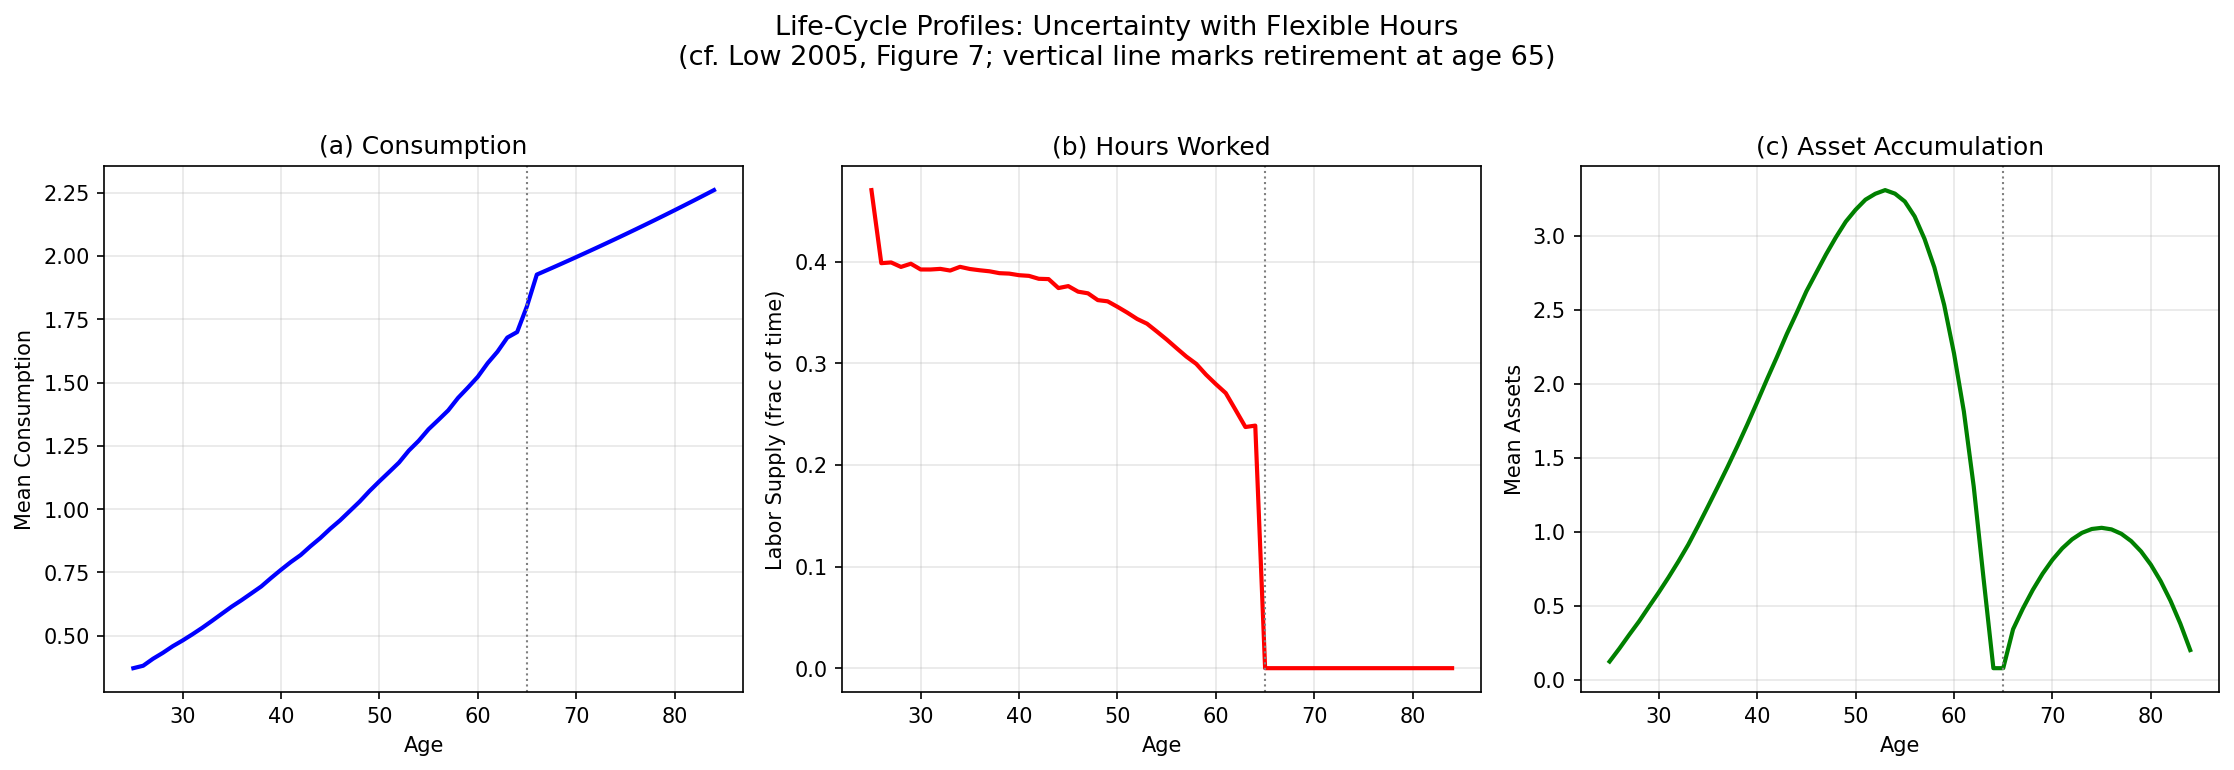
\includegraphics[width=0.95\textwidth]{Figures/lifecycle_profiles.png}
  \caption{Life-cycle profiles of consumption, hours worked, and
  assets for the flexible-hours economy with wage uncertainty
  (cf.\ Low 2005, Figure~7).}
  \label{fig:lifecycle}
\end{figure}

\begin{figure}[htbp]
  \centering
  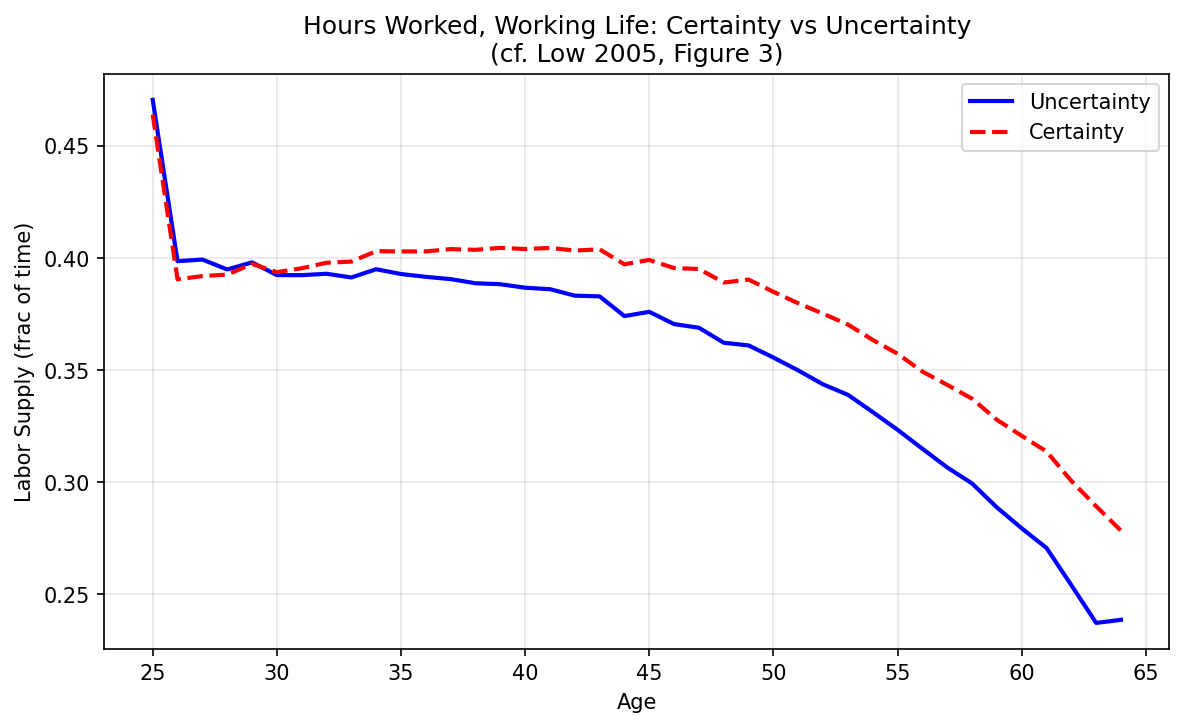
\includegraphics[width=0.75\textwidth]{Figures/hours_cert_vs_uncert.png}
  \caption{Hours worked over the working life under certainty versus
  uncertainty, flexible-hours economy (cf.\ Low 2005, Figure~3).}
  \label{fig:hours-cert-vs-uncert}
\end{figure}

\begin{figure}[htbp]
  \centering
  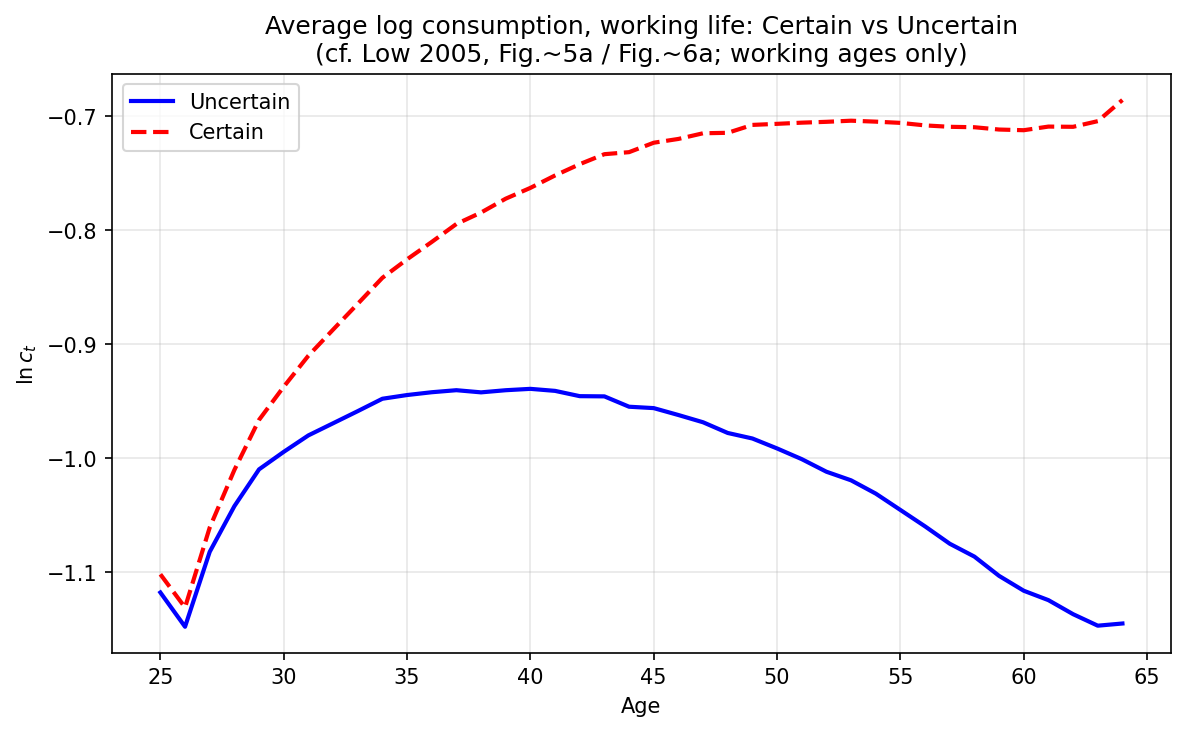
\includegraphics[width=0.75\textwidth]{Figures/consumption_cert_vs_uncert.png}
  \caption{Mean consumption under certainty versus uncertainty,
  flexible-hours economy (cf.\ Low 2005, Figure~4).}
  \label{fig:cons-cert-vs-uncert}
\end{figure}

\begin{figure}[htbp]
  \centering
  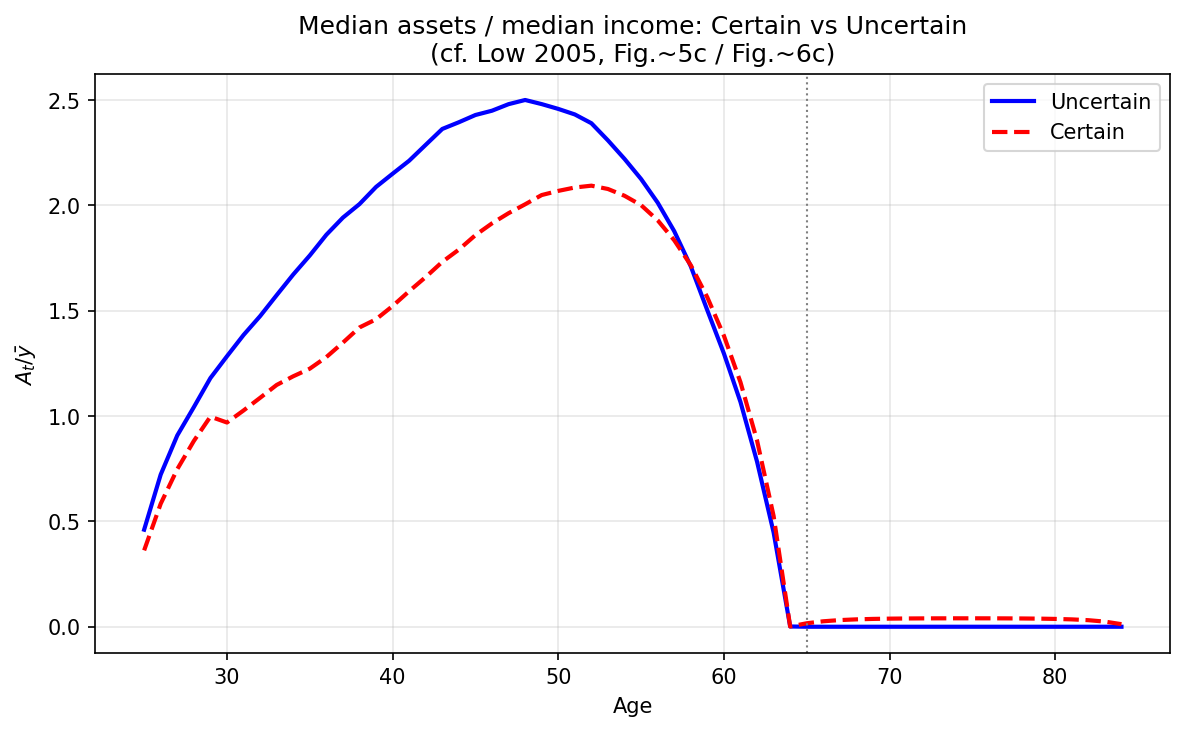
\includegraphics[width=0.75\textwidth]{Figures/assets_cert_vs_uncert.png}
  \caption{Mean asset holdings under certainty versus uncertainty,
  flexible-hours economy (cf.\ Low 2005, Figure~5).}
  \label{fig:assets-cert-vs-uncert}
\end{figure}

\begin{figure}[htbp]
  \centering
  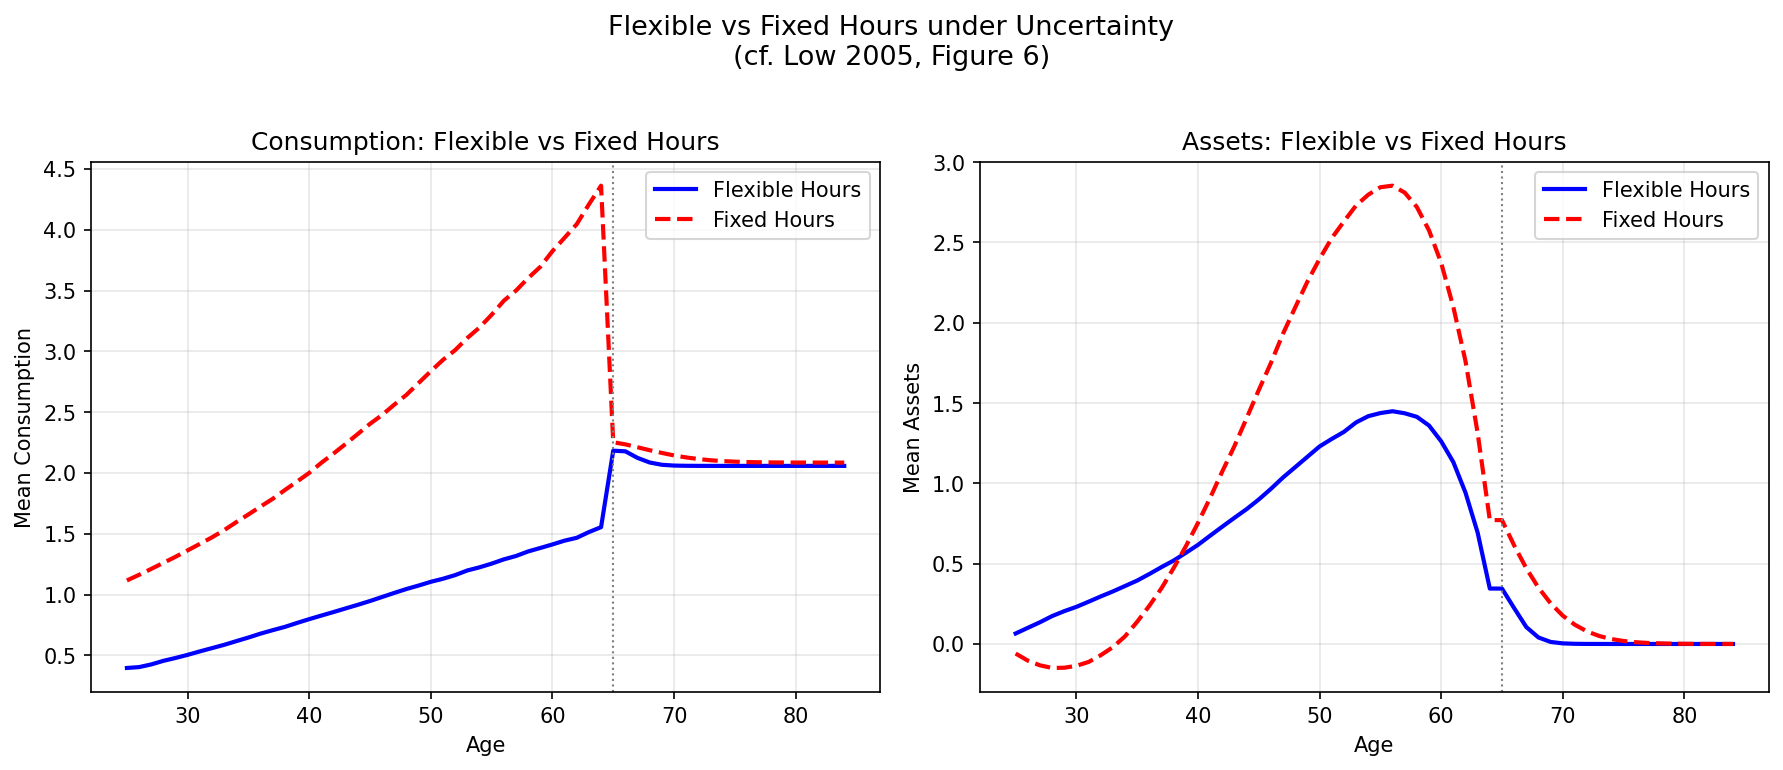
\includegraphics[width=0.95\textwidth]{Figures/flexible_vs_fixed.png}
  \caption{Flexible versus fixed labour supply under wage
  uncertainty: mean consumption and mean assets over the life cycle
  (cf.\ Low 2005, Figure~6).}
  \label{fig:flex-vs-fixed}
\end{figure}

\clearpage

\section{Conclusion}
Low (2005) shows that labour-supply flexibility is an important insurance margin
in life-cycle models with idiosyncratic wage risk. Ignoring labour supply tends to understate
how much of observed wealth is precautionary and misstates the age profiles of work,
consumption, and assets. In the calibrated simulations, flexibility leads households to borrow
more when young, save more in middle age, and produce life-cycle labour profiles that are
closer to the data. This is consistent with later quantitative work such as
\cite{French2004Low}, which also benefits from modelling labour supply jointly with savings
decisions.

\pagebreak

\clearpage
\section*{Appendices}
\addcontentsline{toc}{section}{Appendices}
\markboth{APPENDICES}{APPENDICES}

\appendix
\section{Appendix: Numerical Solution}
The original appendix solves the model recursively by backward induction over the life cycle.
After using the intratemporal first-order condition to express leisure as a function of
consumption and the wage, the dynamic problem can be reduced to solving for the
consumption rule on a finite grid of states. In the paper, expectations are evaluated
numerically and policy functions are interpolated between grid points. The HARK code in
this repository mirrors the economic comparisons of the paper while using modern solution
tools for the corresponding lifecycle household problem.

\end{document}
